\documentclass{article}
\usepackage{lmodern}
\usepackage[T1]{fontenc}
\usepackage{shapepar}
\usepackage{microtype}
\usepackage{lipsum}
\usepackage{pgfplots}
\pgfplotsset{compat=1.9}
\usepackage{tikz}
\usetikzlibrary{calc,fit,intersections,folding}
\usepackage{pstricks-add}
\usetikzlibrary{arrows.meta,angles,arrows,quotes,backgrounds}
\usepackage[a3paper,left=5mm,right=5mm,top=25mm,bottom=25mm]{geometry} % Ränder

\newcommand{\tubecolor}{blue}
\newcommand{\thickness}{0.5mm}
\newcommand{\n}{2.5mm}

\begin{document}
\thispagestyle{empty}
\begin{center}
    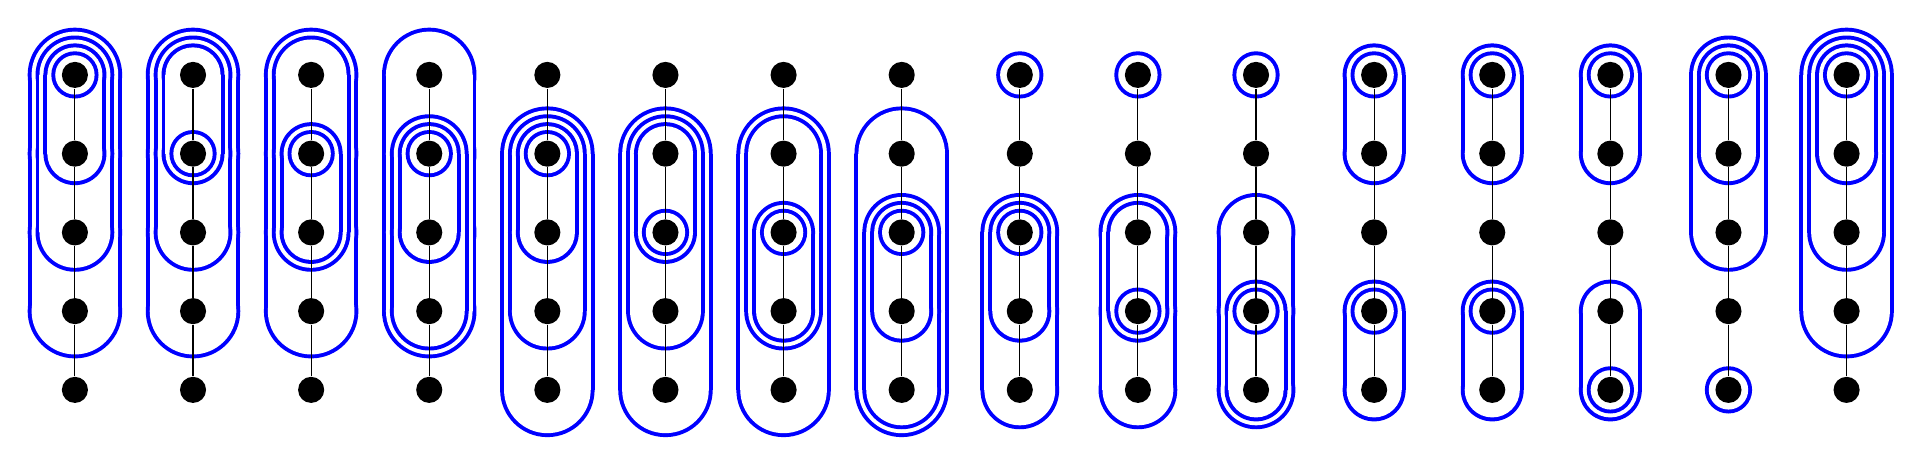
\begin{tikzpicture}
    \begin{scope}
        \node[fill] (1) at (0,4) [circle] {};
        \node[fill] (2) at (0,3) [circle] {};
        \node[fill] (3) at (0,2) [circle] {};
        \node[fill] (4) at (0,1) [circle] {};
        \node[fill] (5) at (0,0) [circle] {};
        \draw (1) -- (2) -- (3) -- (4) -- (5);

        %Tube 1234
        \begin{scope}[on background layer]
            \fill[\tubecolor] (1) circle (\n + 7*\thickness);
            \fill[\tubecolor] (2) circle (\n + 7*\thickness);
            \fill[\tubecolor] (3) circle (\n + 7*\thickness);
            \fill[\tubecolor] (4) circle (\n + 7*\thickness);
            \draw[\tubecolor] [line width = 2*(\n + 7*\thickness)] (1.center) -- (4.center);
            
            \fill[white] (1) circle (\n + 6*\thickness);
            \fill[white] (2) circle (\n + 6*\thickness);
            \fill[white] (3) circle (\n + 6*\thickness);
            \fill[white] (4) circle (\n + 6*\thickness);
            \draw[white] [line width = 2*(\n + 6*\thickness)] (1.center) -- (4.center);
        \end{scope}

        %Tube 123
        \begin{scope}[on background layer]
            \fill[\tubecolor] (1) circle (\n + 5*\thickness);
            \fill[\tubecolor] (2) circle (\n + 5*\thickness);
            \fill[\tubecolor] (3) circle (\n + 5*\thickness);
            \draw[\tubecolor] [line width = 2*(\n + 5*\thickness)] (1.center) -- (3.center);
            
            \fill[white] (1) circle (\n + 4*\thickness);
            \fill[white] (2) circle (\n + 4*\thickness);
            \fill[white] (3) circle (\n + 4*\thickness);
            \draw[white] [line width = 2*(\n + 4*\thickness)] (1.center) -- (3.center);
        \end{scope}
        %Tube 12
        \begin{scope}[on background layer]
            \fill[\tubecolor] (1) circle (\n + 3*\thickness);
            \fill[\tubecolor] (2) circle (\n + 3*\thickness);
            \draw[\tubecolor] [line width = 2*(\n + 3*\thickness)] (1.center) -- (2.center);
            
            \fill[white] (1) circle (\n + 2*\thickness);
            \fill[white] (2) circle (\n + 2*\thickness);
            \draw[white] [line width = 2*(\n + 2*\thickness)] (1.center) -- (2.center);
        \end{scope}
        %Tube 1
        \begin{scope}[on background layer]
            \fill[\tubecolor] (1) circle (\n + 1*\thickness);
            
            \fill[white] (1) circle (\n + 0*\thickness);
        \end{scope}
    \end{scope}

    \begin{scope}[xshift = 1.5cm]
        \node[fill] (1) at (0,4) [circle] {};
        \node[fill] (2) at (0,3) [circle] {};
        \node[fill] (3) at (0,2) [circle] {};
        \node[fill] (4) at (0,1) [circle] {};
        \node[fill] (5) at (0,0) [circle] {};
        \draw (1) -- (2) -- (3) -- (4) -- (5);

        %Tube 1234
        \begin{scope}[on background layer]
            \fill[\tubecolor] (1) circle (\n + 7*\thickness);
            \fill[\tubecolor] (2) circle (\n + 7*\thickness);
            \fill[\tubecolor] (3) circle (\n + 7*\thickness);
            \fill[\tubecolor] (4) circle (\n + 7*\thickness);
            \draw[\tubecolor] [line width = 2*(\n + 7*\thickness)] (1.center) -- (4.center);
            
            \fill[white] (1) circle (\n + 6*\thickness);
            \fill[white] (2) circle (\n + 6*\thickness);
            \fill[white] (3) circle (\n + 6*\thickness);
            \fill[white] (4) circle (\n + 6*\thickness);
            \draw[white] [line width = 2*(\n + 6*\thickness)] (1.center) -- (4.center);
        \end{scope}

        %Tube 123
        \begin{scope}[on background layer]
            \fill[\tubecolor] (1) circle (\n + 5*\thickness);
            \fill[\tubecolor] (2) circle (\n + 5*\thickness);
            \fill[\tubecolor] (3) circle (\n + 5*\thickness);
            \draw[\tubecolor] [line width = 2*(\n + 5*\thickness)] (1.center) -- (3.center);
            
            \fill[white] (1) circle (\n + 4*\thickness);
            \fill[white] (2) circle (\n + 4*\thickness);
            \fill[white] (3) circle (\n + 4*\thickness);
            \draw[white] [line width = 2*(\n + 4*\thickness)] (1.center) -- (3.center);
        \end{scope}
        %Tube 12
        \begin{scope}[on background layer]
            \fill[\tubecolor] (1) circle (\n + 3*\thickness);
            \fill[\tubecolor] (2) circle (\n + 3*\thickness);
            \draw[\tubecolor] [line width = 2*(\n + 3*\thickness)] (1.center) -- (2.center);
            
            \fill[white] (1) circle (\n + 2*\thickness);
            \fill[white] (2) circle (\n + 2*\thickness);
            \draw[white] [line width = 2*(\n + 2*\thickness)] (1.center) -- (2.center);
        \end{scope}
        %Tube 2
        \begin{scope}[on background layer]
            \fill[\tubecolor] (2) circle (\n + 1*\thickness);
            
            \fill[white] (2) circle (\n + 0*\thickness);
        \end{scope}
    \end{scope}

    \begin{scope}[xshift = 3cm]
        \node[fill] (1) at (0,4) [circle] {};
        \node[fill] (2) at (0,3) [circle] {};
        \node[fill] (3) at (0,2) [circle] {};
        \node[fill] (4) at (0,1) [circle] {};
        \node[fill] (5) at (0,0) [circle] {};
        \draw (1) -- (2) -- (3) -- (4) -- (5);

        %Tube 1234
        \begin{scope}[on background layer]
            \fill[\tubecolor] (1) circle (\n + 7*\thickness);
            \fill[\tubecolor] (2) circle (\n + 7*\thickness);
            \fill[\tubecolor] (3) circle (\n + 7*\thickness);
            \fill[\tubecolor] (4) circle (\n + 7*\thickness);
            \draw[\tubecolor] [line width = 2*(\n + 7*\thickness)] (1.center) -- (4.center);
            
            \fill[white] (1) circle (\n + 6*\thickness);
            \fill[white] (2) circle (\n + 6*\thickness);
            \fill[white] (3) circle (\n + 6*\thickness);
            \fill[white] (4) circle (\n + 6*\thickness);
            \draw[white] [line width = 2*(\n + 6*\thickness)] (1.center) -- (4.center);
        \end{scope}

        %Tube 123
        \begin{scope}[on background layer]
            \fill[\tubecolor] (1) circle (\n + 5*\thickness);
            \fill[\tubecolor] (2) circle (\n + 5*\thickness);
            \fill[\tubecolor] (3) circle (\n + 5*\thickness);
            \draw[\tubecolor] [line width = 2*(\n + 5*\thickness)] (1.center) -- (3.center);
            
            \fill[white] (1) circle (\n + 4*\thickness);
            \fill[white] (2) circle (\n + 4*\thickness);
            \fill[white] (3) circle (\n + 4*\thickness);
            \draw[white] [line width = 2*(\n + 4*\thickness)] (1.center) -- (3.center);
        \end{scope}
        %Tube 23
        \begin{scope}[on background layer]
            \fill[\tubecolor] (3) circle (\n + 3*\thickness);
            \fill[\tubecolor] (2) circle (\n + 3*\thickness);
            \draw[\tubecolor] [line width = 2*(\n + 3*\thickness)] (3.center) -- (2.center);
            
            \fill[white] (3) circle (\n + 2*\thickness);
            \fill[white] (2) circle (\n + 2*\thickness);
            \draw[white] [line width = 2*(\n + 2*\thickness)] (3.center) -- (2.center);
        \end{scope}
        %Tube 2
        \begin{scope}[on background layer]
            \fill[\tubecolor] (2) circle (\n + 1*\thickness);
            
            \fill[white] (2) circle (\n + 0*\thickness);
        \end{scope}
    \end{scope}

    \begin{scope}[xshift = 4.5cm]
        \node[fill] (1) at (0,4) [circle] {};
        \node[fill] (2) at (0,3) [circle] {};
        \node[fill] (3) at (0,2) [circle] {};
        \node[fill] (4) at (0,1) [circle] {};
        \node[fill] (5) at (0,0) [circle] {};
        \draw (1) -- (2) -- (3) -- (4) -- (5);

        %Tube 1234
        \begin{scope}[on background layer]
            \fill[\tubecolor] (1) circle (\n + 7*\thickness);
            \fill[\tubecolor] (2) circle (\n + 7*\thickness);
            \fill[\tubecolor] (3) circle (\n + 7*\thickness);
            \fill[\tubecolor] (4) circle (\n + 7*\thickness);
            \draw[\tubecolor] [line width = 2*(\n + 7*\thickness)] (1.center) -- (4.center);
            
            \fill[white] (1) circle (\n + 6*\thickness);
            \fill[white] (2) circle (\n + 6*\thickness);
            \fill[white] (3) circle (\n + 6*\thickness);
            \fill[white] (4) circle (\n + 6*\thickness);
            \draw[white] [line width = 2*(\n + 6*\thickness)] (1.center) -- (4.center);
        \end{scope}

        %Tube 234
        \begin{scope}[on background layer]
            \fill[\tubecolor] (4) circle (\n + 5*\thickness);
            \fill[\tubecolor] (2) circle (\n + 5*\thickness);
            \fill[\tubecolor] (3) circle (\n + 5*\thickness);
            \draw[\tubecolor] [line width = 2*(\n + 5*\thickness)] (2.center) -- (4.center);
            
            \fill[white] (4) circle (\n + 4*\thickness);
            \fill[white] (2) circle (\n + 4*\thickness);
            \fill[white] (3) circle (\n + 4*\thickness);
            \draw[white] [line width = 2*(\n + 4*\thickness)] (2.center) -- (4.center);
        \end{scope}
        %Tube 23
        \begin{scope}[on background layer]
            \fill[\tubecolor] (3) circle (\n + 3*\thickness);
            \fill[\tubecolor] (2) circle (\n + 3*\thickness);
            \draw[\tubecolor] [line width = 2*(\n + 3*\thickness)] (3.center) -- (2.center);
            
            \fill[white] (3) circle (\n + 2*\thickness);
            \fill[white] (2) circle (\n + 2*\thickness);
            \draw[white] [line width = 2*(\n + 2*\thickness)] (3.center) -- (2.center);
        \end{scope}
        %Tube 2
        \begin{scope}[on background layer]
            \fill[\tubecolor] (2) circle (\n + 1*\thickness);
            
            \fill[white] (2) circle (\n + 0*\thickness);
        \end{scope}
    \end{scope}

    \begin{scope}[xshift = 6cm]
        \node[fill] (1) at (0,4) [circle] {};
        \node[fill] (2) at (0,3) [circle] {};
        \node[fill] (3) at (0,2) [circle] {};
        \node[fill] (4) at (0,1) [circle] {};
        \node[fill] (5) at (0,0) [circle] {};
        \draw (1) -- (2) -- (3) -- (4) -- (5);

        %Tube 2345
        \begin{scope}[on background layer]
            \fill[\tubecolor] (5) circle (\n + 7*\thickness);
            \fill[\tubecolor] (2) circle (\n + 7*\thickness);
            \fill[\tubecolor] (3) circle (\n + 7*\thickness);
            \fill[\tubecolor] (4) circle (\n + 7*\thickness);
            \draw[\tubecolor] [line width = 2*(\n + 7*\thickness)] (2.center) -- (5.center);
            
            \fill[white] (5) circle (\n + 6*\thickness);
            \fill[white] (2) circle (\n + 6*\thickness);
            \fill[white] (3) circle (\n + 6*\thickness);
            \fill[white] (4) circle (\n + 6*\thickness);
            \draw[white] [line width = 2*(\n + 6*\thickness)] (2.center) -- (5.center);
        \end{scope}

        %Tube 234
        \begin{scope}[on background layer]
            \fill[\tubecolor] (4) circle (\n + 5*\thickness);
            \fill[\tubecolor] (2) circle (\n + 5*\thickness);
            \fill[\tubecolor] (3) circle (\n + 5*\thickness);
            \draw[\tubecolor] [line width = 2*(\n + 5*\thickness)] (2.center) -- (4.center);
            
            \fill[white] (4) circle (\n + 4*\thickness);
            \fill[white] (2) circle (\n + 4*\thickness);
            \fill[white] (3) circle (\n + 4*\thickness);
            \draw[white] [line width = 2*(\n + 4*\thickness)] (2.center) -- (4.center);
        \end{scope}
        %Tube 23
        \begin{scope}[on background layer]
            \fill[\tubecolor] (3) circle (\n + 3*\thickness);
            \fill[\tubecolor] (2) circle (\n + 3*\thickness);
            \draw[\tubecolor] [line width = 2*(\n + 3*\thickness)] (3.center) -- (2.center);
            
            \fill[white] (3) circle (\n + 2*\thickness);
            \fill[white] (2) circle (\n + 2*\thickness);
            \draw[white] [line width = 2*(\n + 2*\thickness)] (3.center) -- (2.center);
        \end{scope}
        %Tube 2
        \begin{scope}[on background layer]
            \fill[\tubecolor] (2) circle (\n + 1*\thickness);
            
            \fill[white] (2) circle (\n + 0*\thickness);
        \end{scope}
    \end{scope}
    
    \begin{scope}[xshift = 7.5cm]
        \node[fill] (1) at (0,4) [circle] {};
        \node[fill] (2) at (0,3) [circle] {};
        \node[fill] (3) at (0,2) [circle] {};
        \node[fill] (4) at (0,1) [circle] {};
        \node[fill] (5) at (0,0) [circle] {};
        \draw (1) -- (2) -- (3) -- (4) -- (5);

        %Tube 2345
        \begin{scope}[on background layer]
            \fill[\tubecolor] (5) circle (\n + 7*\thickness);
            \fill[\tubecolor] (2) circle (\n + 7*\thickness);
            \fill[\tubecolor] (3) circle (\n + 7*\thickness);
            \fill[\tubecolor] (4) circle (\n + 7*\thickness);
            \draw[\tubecolor] [line width = 2*(\n + 7*\thickness)] (2.center) -- (5.center);
            
            \fill[white] (5) circle (\n + 6*\thickness);
            \fill[white] (2) circle (\n + 6*\thickness);
            \fill[white] (3) circle (\n + 6*\thickness);
            \fill[white] (4) circle (\n + 6*\thickness);
            \draw[white] [line width = 2*(\n + 6*\thickness)] (2.center) -- (5.center);
        \end{scope}

        %Tube 234
        \begin{scope}[on background layer]
            \fill[\tubecolor] (4) circle (\n + 5*\thickness);
            \fill[\tubecolor] (2) circle (\n + 5*\thickness);
            \fill[\tubecolor] (3) circle (\n + 5*\thickness);
            \draw[\tubecolor] [line width = 2*(\n + 5*\thickness)] (2.center) -- (4.center);
            
            \fill[white] (4) circle (\n + 4*\thickness);
            \fill[white] (2) circle (\n + 4*\thickness);
            \fill[white] (3) circle (\n + 4*\thickness);
            \draw[white] [line width = 2*(\n + 4*\thickness)] (2.center) -- (4.center);
        \end{scope}
        %Tube 23
        \begin{scope}[on background layer]
            \fill[\tubecolor] (3) circle (\n + 3*\thickness);
            \fill[\tubecolor] (2) circle (\n + 3*\thickness);
            \draw[\tubecolor] [line width = 2*(\n + 3*\thickness)] (3.center) -- (2.center);
            
            \fill[white] (3) circle (\n + 2*\thickness);
            \fill[white] (2) circle (\n + 2*\thickness);
            \draw[white] [line width = 2*(\n + 2*\thickness)] (3.center) -- (2.center);
        \end{scope}
        %Tube 3
        \begin{scope}[on background layer]
            \fill[\tubecolor] (3) circle (\n + 1*\thickness);
            
            \fill[white] (3) circle (\n + 0*\thickness);
        \end{scope}
    \end{scope}
    
    \begin{scope}[xshift = 9cm]
        \node[fill] (1) at (0,4) [circle] {};
        \node[fill] (2) at (0,3) [circle] {};
        \node[fill] (3) at (0,2) [circle] {};
        \node[fill] (4) at (0,1) [circle] {};
        \node[fill] (5) at (0,0) [circle] {};
        \draw (1) -- (2) -- (3) -- (4) -- (5);

        %Tube 2345
        \begin{scope}[on background layer]
            \fill[\tubecolor] (5) circle (\n + 7*\thickness);
            \fill[\tubecolor] (2) circle (\n + 7*\thickness);
            \fill[\tubecolor] (3) circle (\n + 7*\thickness);
            \fill[\tubecolor] (4) circle (\n + 7*\thickness);
            \draw[\tubecolor] [line width = 2*(\n + 7*\thickness)] (2.center) -- (5.center);
            
            \fill[white] (5) circle (\n + 6*\thickness);
            \fill[white] (2) circle (\n + 6*\thickness);
            \fill[white] (3) circle (\n + 6*\thickness);
            \fill[white] (4) circle (\n + 6*\thickness);
            \draw[white] [line width = 2*(\n + 6*\thickness)] (2.center) -- (5.center);
        \end{scope}

        %Tube 234
        \begin{scope}[on background layer]
            \fill[\tubecolor] (4) circle (\n + 5*\thickness);
            \fill[\tubecolor] (2) circle (\n + 5*\thickness);
            \fill[\tubecolor] (3) circle (\n + 5*\thickness);
            \draw[\tubecolor] [line width = 2*(\n + 5*\thickness)] (2.center) -- (4.center);
            
            \fill[white] (4) circle (\n + 4*\thickness);
            \fill[white] (2) circle (\n + 4*\thickness);
            \fill[white] (3) circle (\n + 4*\thickness);
            \draw[white] [line width = 2*(\n + 4*\thickness)] (2.center) -- (4.center);
        \end{scope}
        %Tube 34
        \begin{scope}[on background layer]
            \fill[\tubecolor] (3) circle (\n + 3*\thickness);
            \fill[\tubecolor] (4) circle (\n + 3*\thickness);
            \draw[\tubecolor] [line width = 2*(\n + 3*\thickness)] (3.center) -- (4.center);
            
            \fill[white] (3) circle (\n + 2*\thickness);
            \fill[white] (4) circle (\n + 2*\thickness);
            \draw[white] [line width = 2*(\n + 2*\thickness)] (3.center) -- (4.center);
        \end{scope}
        %Tube 3
        \begin{scope}[on background layer]
            \fill[\tubecolor] (3) circle (\n + 1*\thickness);
            
            \fill[white] (3) circle (\n + 0*\thickness);
        \end{scope}
    \end{scope}

    \begin{scope}[xshift = 10.5cm]
        \node[fill] (1) at (0,4) [circle] {};
        \node[fill] (2) at (0,3) [circle] {};
        \node[fill] (3) at (0,2) [circle] {};
        \node[fill] (4) at (0,1) [circle] {};
        \node[fill] (5) at (0,0) [circle] {};
        \draw (1) -- (2) -- (3) -- (4) -- (5);

        %Tube 2345
        \begin{scope}[on background layer]
            \fill[\tubecolor] (5) circle (\n + 7*\thickness);
            \fill[\tubecolor] (2) circle (\n + 7*\thickness);
            \fill[\tubecolor] (3) circle (\n + 7*\thickness);
            \fill[\tubecolor] (4) circle (\n + 7*\thickness);
            \draw[\tubecolor] [line width = 2*(\n + 7*\thickness)] (2.center) -- (5.center);
            
            \fill[white] (5) circle (\n + 6*\thickness);
            \fill[white] (2) circle (\n + 6*\thickness);
            \fill[white] (3) circle (\n + 6*\thickness);
            \fill[white] (4) circle (\n + 6*\thickness);
            \draw[white] [line width = 2*(\n + 6*\thickness)] (2.center) -- (5.center);
        \end{scope}

        %Tube 345
        \begin{scope}[on background layer]
            \fill[\tubecolor] (4) circle (\n + 5*\thickness);
            \fill[\tubecolor] (5) circle (\n + 5*\thickness);
            \fill[\tubecolor] (3) circle (\n + 5*\thickness);
            \draw[\tubecolor] [line width = 2*(\n + 5*\thickness)] (3.center) -- (5.center);
            
            \fill[white] (4) circle (\n + 4*\thickness);
            \fill[white] (5) circle (\n + 4*\thickness);
            \fill[white] (3) circle (\n + 4*\thickness);
            \draw[white] [line width = 2*(\n + 4*\thickness)] (3.center) -- (5.center);
        \end{scope}
        %Tube 34
        \begin{scope}[on background layer]
            \fill[\tubecolor] (3) circle (\n + 3*\thickness);
            \fill[\tubecolor] (4) circle (\n + 3*\thickness);
            \draw[\tubecolor] [line width = 2*(\n + 3*\thickness)] (3.center) -- (4.center);
            
            \fill[white] (3) circle (\n + 2*\thickness);
            \fill[white] (4) circle (\n + 2*\thickness);
            \draw[white] [line width = 2*(\n + 2*\thickness)] (3.center) -- (4.center);
        \end{scope}
        %Tube 3
        \begin{scope}[on background layer]
            \fill[\tubecolor] (3) circle (\n + 1*\thickness);
            
            \fill[white] (3) circle (\n + 0*\thickness);
        \end{scope}
    \end{scope}

    \begin{scope}[xshift = 12cm]
        \node[fill] (1) at (0,4) [circle] {};
        \node[fill] (2) at (0,3) [circle] {};
        \node[fill] (3) at (0,2) [circle] {};
        \node[fill] (4) at (0,1) [circle] {};
        \node[fill] (5) at (0,0) [circle] {};
        \draw (1) -- (2) -- (3) -- (4) -- (5);

        %Tube 1
        \begin{scope}[on background layer]
            \fill[\tubecolor] (1) circle (\n + 1*\thickness);
            
            \fill[white] (1) circle (\n + 0*\thickness);
        \end{scope}

        %Tube 345
        \begin{scope}[on background layer]
            \fill[\tubecolor] (4) circle (\n + 5*\thickness);
            \fill[\tubecolor] (5) circle (\n + 5*\thickness);
            \fill[\tubecolor] (3) circle (\n + 5*\thickness);
            \draw[\tubecolor] [line width = 2*(\n + 5*\thickness)] (3.center) -- (5.center);
            
            \fill[white] (4) circle (\n + 4*\thickness);
            \fill[white] (5) circle (\n + 4*\thickness);
            \fill[white] (3) circle (\n + 4*\thickness);
            \draw[white] [line width = 2*(\n + 4*\thickness)] (3.center) -- (5.center);
        \end{scope}
        %Tube 34
        \begin{scope}[on background layer]
            \fill[\tubecolor] (3) circle (\n + 3*\thickness);
            \fill[\tubecolor] (4) circle (\n + 3*\thickness);
            \draw[\tubecolor] [line width = 2*(\n + 3*\thickness)] (3.center) -- (4.center);
            
            \fill[white] (3) circle (\n + 2*\thickness);
            \fill[white] (4) circle (\n + 2*\thickness);
            \draw[white] [line width = 2*(\n + 2*\thickness)] (3.center) -- (4.center);
        \end{scope}
        %Tube 3
        \begin{scope}[on background layer]
            \fill[\tubecolor] (3) circle (\n + 1*\thickness);
            
            \fill[white] (3) circle (\n + 0*\thickness);
        \end{scope}
    \end{scope}

    \begin{scope}[xshift = 13.5cm]
        \node[fill] (1) at (0,4) [circle] {};
        \node[fill] (2) at (0,3) [circle] {};
        \node[fill] (3) at (0,2) [circle] {};
        \node[fill] (4) at (0,1) [circle] {};
        \node[fill] (5) at (0,0) [circle] {};
        \draw (1) -- (2) -- (3) -- (4) -- (5);

        %Tube 1
        \begin{scope}[on background layer]
            \fill[\tubecolor] (1) circle (\n + 1*\thickness);
            
            \fill[white] (1) circle (\n + 0*\thickness);
        \end{scope}

        %Tube 345
        \begin{scope}[on background layer]
            \fill[\tubecolor] (4) circle (\n + 5*\thickness);
            \fill[\tubecolor] (5) circle (\n + 5*\thickness);
            \fill[\tubecolor] (3) circle (\n + 5*\thickness);
            \draw[\tubecolor] [line width = 2*(\n + 5*\thickness)] (3.center) -- (5.center);
            
            \fill[white] (4) circle (\n + 4*\thickness);
            \fill[white] (5) circle (\n + 4*\thickness);
            \fill[white] (3) circle (\n + 4*\thickness);
            \draw[white] [line width = 2*(\n + 4*\thickness)] (3.center) -- (5.center);
        \end{scope}
        %Tube 34
        \begin{scope}[on background layer]
            \fill[\tubecolor] (3) circle (\n + 3*\thickness);
            \fill[\tubecolor] (4) circle (\n + 3*\thickness);
            \draw[\tubecolor] [line width = 2*(\n + 3*\thickness)] (3.center) -- (4.center);
            
            \fill[white] (3) circle (\n + 2*\thickness);
            \fill[white] (4) circle (\n + 2*\thickness);
            \draw[white] [line width = 2*(\n + 2*\thickness)] (3.center) -- (4.center);
        \end{scope}
        %Tube 4
        \begin{scope}[on background layer]
            \fill[\tubecolor] (4) circle (\n + 1*\thickness);
            
            \fill[white] (4) circle (\n + 0*\thickness);
        \end{scope}
    \end{scope}

    \begin{scope}[xshift = 15cm]
        \node[fill] (1) at (0,4) [circle] {};
        \node[fill] (2) at (0,3) [circle] {};
        \node[fill] (3) at (0,2) [circle] {};
        \node[fill] (4) at (0,1) [circle] {};
        \node[fill] (5) at (0,0) [circle] {};
        \draw (1) -- (2) -- (3) -- (4) -- (5);

        %Tube 1
        \begin{scope}[on background layer]
            \fill[\tubecolor] (1) circle (\n + 1*\thickness);
            
            \fill[white] (1) circle (\n + 0*\thickness);
        \end{scope}

        %Tube 345
        \begin{scope}[on background layer]
            \fill[\tubecolor] (4) circle (\n + 5*\thickness);
            \fill[\tubecolor] (5) circle (\n + 5*\thickness);
            \fill[\tubecolor] (3) circle (\n + 5*\thickness);
            \draw[\tubecolor] [line width = 2*(\n + 5*\thickness)] (3.center) -- (5.center);
            
            \fill[white] (4) circle (\n + 4*\thickness);
            \fill[white] (5) circle (\n + 4*\thickness);
            \fill[white] (3) circle (\n + 4*\thickness);
            \draw[white] [line width = 2*(\n + 4*\thickness)] (3.center) -- (5.center);
        \end{scope}
        %Tube 45
        \begin{scope}[on background layer]
            \fill[\tubecolor] (5) circle (\n + 3*\thickness);
            \fill[\tubecolor] (4) circle (\n + 3*\thickness);
            \draw[\tubecolor] [line width = 2*(\n + 3*\thickness)] (5.center) -- (4.center);
            
            \fill[white] (5) circle (\n + 2*\thickness);
            \fill[white] (4) circle (\n + 2*\thickness);
            \draw[white] [line width = 2*(\n + 2*\thickness)] (5.center) -- (4.center);
        \end{scope}
        %Tube 4
        \begin{scope}[on background layer]
            \fill[\tubecolor] (4) circle (\n + 1*\thickness);
            
            \fill[white] (4) circle (\n + 0*\thickness);
        \end{scope}
    \end{scope}

    \begin{scope}[xshift = 16.5cm]
        \node[fill] (1) at (0,4) [circle] {};
        \node[fill] (2) at (0,3) [circle] {};
        \node[fill] (3) at (0,2) [circle] {};
        \node[fill] (4) at (0,1) [circle] {};
        \node[fill] (5) at (0,0) [circle] {};
        \draw (1) -- (2) -- (3) -- (4) -- (5);

       

        %Tube 12
        \begin{scope}[on background layer]
            \fill[\tubecolor] (1) circle (\n + 3*\thickness);
            \fill[\tubecolor] (2) circle (\n + 3*\thickness);
            \draw[\tubecolor] [line width = 2*(\n + 3*\thickness)] (1.center) -- (2.center);
            
            \fill[white] (1) circle (\n + 2*\thickness);
            \fill[white] (2) circle (\n + 2*\thickness);
            \draw[white] [line width = 2*(\n + 2*\thickness)] (1.center) -- (2.center);
        \end{scope}
        %Tube 45
        \begin{scope}[on background layer]
            \fill[\tubecolor] (5) circle (\n + 3*\thickness);
            \fill[\tubecolor] (4) circle (\n + 3*\thickness);
            \draw[\tubecolor] [line width = 2*(\n + 3*\thickness)] (5.center) -- (4.center);
            
            \fill[white] (5) circle (\n + 2*\thickness);
            \fill[white] (4) circle (\n + 2*\thickness);
            \draw[white] [line width = 2*(\n + 2*\thickness)] (5.center) -- (4.center);
        \end{scope}
        %Tube 1
        \begin{scope}[on background layer]
            \fill[\tubecolor] (1) circle (\n + 1*\thickness);
            
            \fill[white] (1) circle (\n + 0*\thickness);
        \end{scope}
        %Tube 4
        \begin{scope}[on background layer]
            \fill[\tubecolor] (4) circle (\n + 1*\thickness);
            
            \fill[white] (4) circle (\n + 0*\thickness);
        \end{scope}
    \end{scope}
    
    \begin{scope}[xshift = 18cm]
        \node[fill] (1) at (0,4) [circle] {};
        \node[fill] (2) at (0,3) [circle] {};
        \node[fill] (3) at (0,2) [circle] {};
        \node[fill] (4) at (0,1) [circle] {};
        \node[fill] (5) at (0,0) [circle] {};
        \draw (1) -- (2) -- (3) -- (4) -- (5);

        %Tube 12
        \begin{scope}[on background layer]
            \fill[\tubecolor] (1) circle (\n + 3*\thickness);
            \fill[\tubecolor] (2) circle (\n + 3*\thickness);
            \draw[\tubecolor] [line width = 2*(\n + 3*\thickness)] (1.center) -- (2.center);
            
            \fill[white] (1) circle (\n + 2*\thickness);
            \fill[white] (2) circle (\n + 2*\thickness);
            \draw[white] [line width = 2*(\n + 2*\thickness)] (1.center) -- (2.center);
        \end{scope}
        
        %Tube 45
        \begin{scope}[on background layer]
            \fill[\tubecolor] (5) circle (\n + 3*\thickness);
            \fill[\tubecolor] (4) circle (\n + 3*\thickness);
            \draw[\tubecolor] [line width = 2*(\n + 3*\thickness)] (5.center) -- (4.center);
            
            \fill[white] (5) circle (\n + 2*\thickness);
            \fill[white] (4) circle (\n + 2*\thickness);
            \draw[white] [line width = 2*(\n + 2*\thickness)] (5.center) -- (4.center);
        \end{scope}
        %Tube 1
        \begin{scope}[on background layer]
            \fill[\tubecolor] (1) circle (\n + 1*\thickness);
            
            \fill[white] (1) circle (\n + 0*\thickness);
        \end{scope}
        %Tube 4
        \begin{scope}[on background layer]
            \fill[\tubecolor] (4) circle (\n + 1*\thickness);
            
            \fill[white] (4) circle (\n + 0*\thickness);
        \end{scope}
    \end{scope}
    
    \begin{scope}[xshift = 19.5cm]
        \node[fill] (1) at (0,4) [circle] {};
        \node[fill] (2) at (0,3) [circle] {};
        \node[fill] (3) at (0,2) [circle] {};
        \node[fill] (4) at (0,1) [circle] {};
        \node[fill] (5) at (0,0) [circle] {};
        \draw (1) -- (2) -- (3) -- (4) -- (5);

        %Tube 12
        \begin{scope}[on background layer]
            \fill[\tubecolor] (1) circle (\n + 3*\thickness);
            \fill[\tubecolor] (2) circle (\n + 3*\thickness);
            \draw[\tubecolor] [line width = 2*(\n + 3*\thickness)] (1.center) -- (2.center);
            
            \fill[white] (1) circle (\n + 2*\thickness);
            \fill[white] (2) circle (\n + 2*\thickness);
            \draw[white] [line width = 2*(\n + 2*\thickness)] (1.center) -- (2.center);
        \end{scope}
        
        %Tube 45
        \begin{scope}[on background layer]
            \fill[\tubecolor] (5) circle (\n + 3*\thickness);
            \fill[\tubecolor] (4) circle (\n + 3*\thickness);
            \draw[\tubecolor] [line width = 2*(\n + 3*\thickness)] (5.center) -- (4.center);
            
            \fill[white] (5) circle (\n + 2*\thickness);
            \fill[white] (4) circle (\n + 2*\thickness);
            \draw[white] [line width = 2*(\n + 2*\thickness)] (5.center) -- (4.center);
        \end{scope}
        %Tube 1
        \begin{scope}[on background layer]
            \fill[\tubecolor] (1) circle (\n + 1*\thickness);
            
            \fill[white] (1) circle (\n + 0*\thickness);
        \end{scope}
        %Tube 5
        \begin{scope}[on background layer]
            \fill[\tubecolor] (5) circle (\n + 1*\thickness);
            
            \fill[white] (5) circle (\n + 0*\thickness);
        \end{scope}
    \end{scope}

    \begin{scope}[xshift = 21cm]
        \node[fill] (1) at (0,4) [circle] {};
        \node[fill] (2) at (0,3) [circle] {};
        \node[fill] (3) at (0,2) [circle] {};
        \node[fill] (4) at (0,1) [circle] {};
        \node[fill] (5) at (0,0) [circle] {};
        \draw (1) -- (2) -- (3) -- (4) -- (5);

        %Tube 123
        \begin{scope}[on background layer]
            \fill[\tubecolor] (1) circle (\n + 5*\thickness);
            \fill[\tubecolor] (2) circle (\n + 5*\thickness);
            \fill[\tubecolor] (3) circle (\n + 5*\thickness);
            \draw[\tubecolor] [line width = 2*(\n + 5*\thickness)] (1.center) -- (3.center);
            
            \fill[white] (1) circle (\n + 4*\thickness);
            \fill[white] (2) circle (\n + 4*\thickness);
            \fill[white] (3) circle (\n + 4*\thickness);
            \draw[white] [line width = 2*(\n + 4*\thickness)] (1.center) -- (3.center);
        \end{scope}
        %Tube 12
        \begin{scope}[on background layer]
            \fill[\tubecolor] (1) circle (\n + 3*\thickness);
            \fill[\tubecolor] (2) circle (\n + 3*\thickness);
            \draw[\tubecolor] [line width = 2*(\n + 3*\thickness)] (1.center) -- (2.center);
            
            \fill[white] (1) circle (\n + 2*\thickness);
            \fill[white] (2) circle (\n + 2*\thickness);
            \draw[white] [line width = 2*(\n + 2*\thickness)] (1.center) -- (2.center);
        \end{scope}
        %Tube 1
        \begin{scope}[on background layer]
            \fill[\tubecolor] (1) circle (\n + 1*\thickness);
            
            \fill[white] (1) circle (\n + 0*\thickness);
        \end{scope}
        %Tube 5
        \begin{scope}[on background layer]
            \fill[\tubecolor] (5) circle (\n + 1*\thickness);
            
            \fill[white] (5) circle (\n + 0*\thickness);
        \end{scope}
    \end{scope}

    \begin{scope}[xshift = 22.5cm]
        \node[fill] (1) at (0,4) [circle] {};
        \node[fill] (2) at (0,3) [circle] {};
        \node[fill] (3) at (0,2) [circle] {};
        \node[fill] (4) at (0,1) [circle] {};
        \node[fill] (5) at (0,0) [circle] {};
        \draw (1) -- (2) -- (3) -- (4) -- (5);

        %Tube 1234
        \begin{scope}[on background layer]
            \fill[\tubecolor] (1) circle (\n + 7*\thickness);
            \fill[\tubecolor] (2) circle (\n + 7*\thickness);
            \fill[\tubecolor] (3) circle (\n + 7*\thickness);
            \fill[\tubecolor] (4) circle (\n + 7*\thickness);
            \draw[\tubecolor] [line width = 2*(\n + 7*\thickness)] (1.center) -- (4.center);
            
            \fill[white] (1) circle (\n + 6*\thickness);
            \fill[white] (2) circle (\n + 6*\thickness);
            \fill[white] (3) circle (\n + 6*\thickness);
            \fill[white] (4) circle (\n + 6*\thickness);
            \draw[white] [line width = 2*(\n + 6*\thickness)] (1.center) -- (4.center);
        \end{scope}

        %Tube 123
        \begin{scope}[on background layer]
            \fill[\tubecolor] (1) circle (\n + 5*\thickness);
            \fill[\tubecolor] (2) circle (\n + 5*\thickness);
            \fill[\tubecolor] (3) circle (\n + 5*\thickness);
            \draw[\tubecolor] [line width = 2*(\n + 5*\thickness)] (1.center) -- (3.center);
            
            \fill[white] (1) circle (\n + 4*\thickness);
            \fill[white] (2) circle (\n + 4*\thickness);
            \fill[white] (3) circle (\n + 4*\thickness);
            \draw[white] [line width = 2*(\n + 4*\thickness)] (1.center) -- (3.center);
        \end{scope}
        %Tube 12
        \begin{scope}[on background layer]
            \fill[\tubecolor] (1) circle (\n + 3*\thickness);
            \fill[\tubecolor] (2) circle (\n + 3*\thickness);
            \draw[\tubecolor] [line width = 2*(\n + 3*\thickness)] (1.center) -- (2.center);
            
            \fill[white] (1) circle (\n + 2*\thickness);
            \fill[white] (2) circle (\n + 2*\thickness);
            \draw[white] [line width = 2*(\n + 2*\thickness)] (1.center) -- (2.center);
        \end{scope}
        %Tube 1
        \begin{scope}[on background layer]
            \fill[\tubecolor] (1) circle (\n + 1*\thickness);
            
            \fill[white] (1) circle (\n + 0*\thickness);
        \end{scope}
    \end{scope}
\end{tikzpicture}
\end{center}
\end{document}